% Options for packages loaded elsewhere
\PassOptionsToPackage{unicode}{hyperref}
\PassOptionsToPackage{hyphens}{url}
%
\documentclass[
]{article}
\usepackage{amsmath,amssymb}
\usepackage{lmodern}
\usepackage{iftex}
\ifPDFTeX
  \usepackage[T1]{fontenc}
  \usepackage[utf8]{inputenc}
  \usepackage{textcomp} % provide euro and other symbols
\else % if luatex or xetex
  \usepackage{unicode-math}
  \defaultfontfeatures{Scale=MatchLowercase}
  \defaultfontfeatures[\rmfamily]{Ligatures=TeX,Scale=1}
\fi
% Use upquote if available, for straight quotes in verbatim environments
\IfFileExists{upquote.sty}{\usepackage{upquote}}{}
\IfFileExists{microtype.sty}{% use microtype if available
  \usepackage[]{microtype}
  \UseMicrotypeSet[protrusion]{basicmath} % disable protrusion for tt fonts
}{}
\makeatletter
\@ifundefined{KOMAClassName}{% if non-KOMA class
  \IfFileExists{parskip.sty}{%
    \usepackage{parskip}
  }{% else
    \setlength{\parindent}{0pt}
    \setlength{\parskip}{6pt plus 2pt minus 1pt}}
}{% if KOMA class
  \KOMAoptions{parskip=half}}
\makeatother
\usepackage{xcolor}
\usepackage[margin=1in]{geometry}
\usepackage{color}
\usepackage{fancyvrb}
\newcommand{\VerbBar}{|}
\newcommand{\VERB}{\Verb[commandchars=\\\{\}]}
\DefineVerbatimEnvironment{Highlighting}{Verbatim}{commandchars=\\\{\}}
% Add ',fontsize=\small' for more characters per line
\usepackage{framed}
\definecolor{shadecolor}{RGB}{248,248,248}
\newenvironment{Shaded}{\begin{snugshade}}{\end{snugshade}}
\newcommand{\AlertTok}[1]{\textcolor[rgb]{0.94,0.16,0.16}{#1}}
\newcommand{\AnnotationTok}[1]{\textcolor[rgb]{0.56,0.35,0.01}{\textbf{\textit{#1}}}}
\newcommand{\AttributeTok}[1]{\textcolor[rgb]{0.77,0.63,0.00}{#1}}
\newcommand{\BaseNTok}[1]{\textcolor[rgb]{0.00,0.00,0.81}{#1}}
\newcommand{\BuiltInTok}[1]{#1}
\newcommand{\CharTok}[1]{\textcolor[rgb]{0.31,0.60,0.02}{#1}}
\newcommand{\CommentTok}[1]{\textcolor[rgb]{0.56,0.35,0.01}{\textit{#1}}}
\newcommand{\CommentVarTok}[1]{\textcolor[rgb]{0.56,0.35,0.01}{\textbf{\textit{#1}}}}
\newcommand{\ConstantTok}[1]{\textcolor[rgb]{0.00,0.00,0.00}{#1}}
\newcommand{\ControlFlowTok}[1]{\textcolor[rgb]{0.13,0.29,0.53}{\textbf{#1}}}
\newcommand{\DataTypeTok}[1]{\textcolor[rgb]{0.13,0.29,0.53}{#1}}
\newcommand{\DecValTok}[1]{\textcolor[rgb]{0.00,0.00,0.81}{#1}}
\newcommand{\DocumentationTok}[1]{\textcolor[rgb]{0.56,0.35,0.01}{\textbf{\textit{#1}}}}
\newcommand{\ErrorTok}[1]{\textcolor[rgb]{0.64,0.00,0.00}{\textbf{#1}}}
\newcommand{\ExtensionTok}[1]{#1}
\newcommand{\FloatTok}[1]{\textcolor[rgb]{0.00,0.00,0.81}{#1}}
\newcommand{\FunctionTok}[1]{\textcolor[rgb]{0.00,0.00,0.00}{#1}}
\newcommand{\ImportTok}[1]{#1}
\newcommand{\InformationTok}[1]{\textcolor[rgb]{0.56,0.35,0.01}{\textbf{\textit{#1}}}}
\newcommand{\KeywordTok}[1]{\textcolor[rgb]{0.13,0.29,0.53}{\textbf{#1}}}
\newcommand{\NormalTok}[1]{#1}
\newcommand{\OperatorTok}[1]{\textcolor[rgb]{0.81,0.36,0.00}{\textbf{#1}}}
\newcommand{\OtherTok}[1]{\textcolor[rgb]{0.56,0.35,0.01}{#1}}
\newcommand{\PreprocessorTok}[1]{\textcolor[rgb]{0.56,0.35,0.01}{\textit{#1}}}
\newcommand{\RegionMarkerTok}[1]{#1}
\newcommand{\SpecialCharTok}[1]{\textcolor[rgb]{0.00,0.00,0.00}{#1}}
\newcommand{\SpecialStringTok}[1]{\textcolor[rgb]{0.31,0.60,0.02}{#1}}
\newcommand{\StringTok}[1]{\textcolor[rgb]{0.31,0.60,0.02}{#1}}
\newcommand{\VariableTok}[1]{\textcolor[rgb]{0.00,0.00,0.00}{#1}}
\newcommand{\VerbatimStringTok}[1]{\textcolor[rgb]{0.31,0.60,0.02}{#1}}
\newcommand{\WarningTok}[1]{\textcolor[rgb]{0.56,0.35,0.01}{\textbf{\textit{#1}}}}
\usepackage{graphicx}
\makeatletter
\def\maxwidth{\ifdim\Gin@nat@width>\linewidth\linewidth\else\Gin@nat@width\fi}
\def\maxheight{\ifdim\Gin@nat@height>\textheight\textheight\else\Gin@nat@height\fi}
\makeatother
% Scale images if necessary, so that they will not overflow the page
% margins by default, and it is still possible to overwrite the defaults
% using explicit options in \includegraphics[width, height, ...]{}
\setkeys{Gin}{width=\maxwidth,height=\maxheight,keepaspectratio}
% Set default figure placement to htbp
\makeatletter
\def\fps@figure{htbp}
\makeatother
\setlength{\emergencystretch}{3em} % prevent overfull lines
\providecommand{\tightlist}{%
  \setlength{\itemsep}{0pt}\setlength{\parskip}{0pt}}
\setcounter{secnumdepth}{-\maxdimen} % remove section numbering
\ifLuaTeX
  \usepackage{selnolig}  % disable illegal ligatures
\fi
\IfFileExists{bookmark.sty}{\usepackage{bookmark}}{\usepackage{hyperref}}
\IfFileExists{xurl.sty}{\usepackage{xurl}}{} % add URL line breaks if available
\urlstyle{same} % disable monospaced font for URLs
\hypersetup{
  pdftitle={Manipulação de imagens},
  pdfauthor={Artur Almeida, Brenda Assis, Eraldo Jair e Rafael Yui},
  hidelinks,
  pdfcreator={LaTeX via pandoc}}

\title{Manipulação de imagens}
\author{Artur Almeida, Brenda Assis, Eraldo Jair e Rafael Yui}
\date{24 de agosto de 2022}

\begin{document}
\maketitle

\hypertarget{sumuxe1rio}{%
\section{Sumário}\label{sumuxe1rio}}

\tableofcontents

\begin{itemize}
\tightlist
\item
  Introdução

  \begin{itemize}
  \tightlist
  \item
    imagens digitais
  \item
    imagens vetoriais e imagens raster
  \item
    Formatos de imagens -Formatos vetoriais -Formatos raster
  \end{itemize}
\item
  Lendo imagens
\item
  Escrevendo imagens
\item
  Manipulação de constraste
\end{itemize}

\hypertarget{imagens-digitais}{%
\section{imagens digitais}\label{imagens-digitais}}

\begin{itemize}
\item
  imagem é representação visual de uma pessoa ou de um objeto.
\item
  Já imagem digital é a representação de uma imagem bidimensional usando
  números binários codificados de modo a permitir seu armazenamento,
  transferência, impressão ou reprodução, e seu processamento por meios
  eletrônicos.
\item
  Existem dois principais tipos de imagens que podem ser armazenadas em
  um computador: as imagens vetoriais e as imagens raster.
\end{itemize}

\hypertarget{imagens-vetoriais-e-imagens-raster}{%
\section{imagens vetoriais e imagens
raster}\label{imagens-vetoriais-e-imagens-raster}}

\begin{figure}
\centering
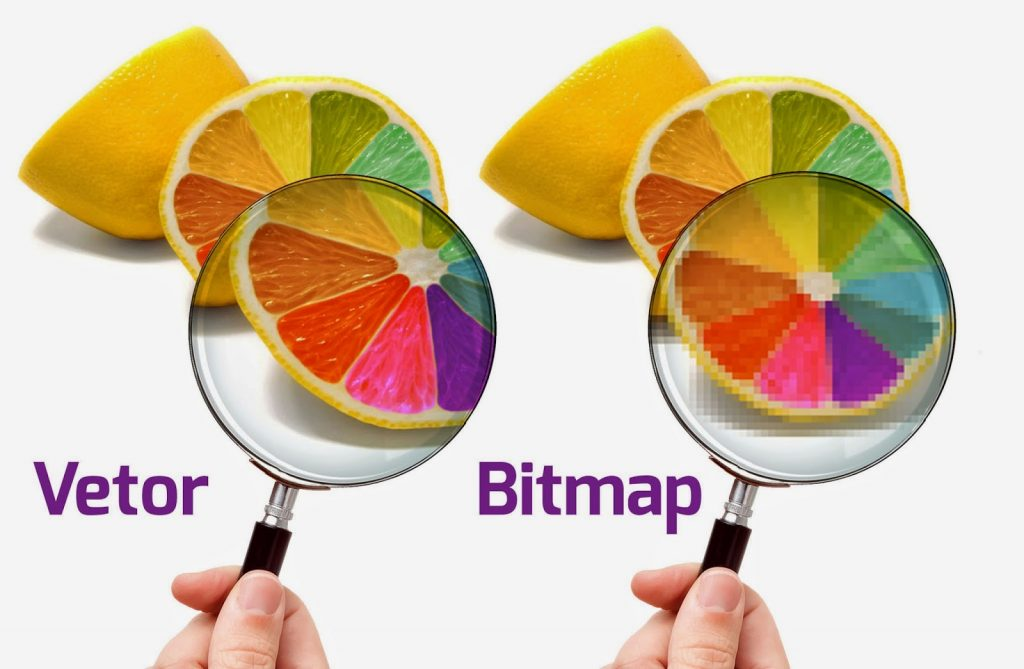
\includegraphics[width=1\textwidth,height=\textheight]{C:/Users/User/OneDrive-unb.br/Documentos/GitHub/Manipulacao-de-imagens/images/vebi.jpg}
\caption{image}
\end{figure}

\hypertarget{formatos-de-imagens}{%
\section{Formatos de imagens}\label{formatos-de-imagens}}

\hypertarget{formatos-vetoriais}{%
\subsection{Formatos vetoriais}\label{formatos-vetoriais}}

\begin{itemize}
\tightlist
\item
  PDF
\item
  PostScript (EPS)
\item
  SVG
\end{itemize}

\hypertarget{formatos-raster}{%
\subsection{Formatos raster}\label{formatos-raster}}

\begin{itemize}
\tightlist
\item
  TIFF
\item
  JPEG
\item
  PNG
\item
  BMP
\item
  PBM
\end{itemize}

\hypertarget{usando-o-pacote-magick}{%
\section{Usando o pacote Magick}\label{usando-o-pacote-magick}}

\hypertarget{leitura}{%
\subsection{Leitura}\label{leitura}}

\begin{Shaded}
\begin{Highlighting}[]
\FunctionTok{library}\NormalTok{(magick)}

\NormalTok{ben }\OtherTok{\textless{}{-}} \FunctionTok{image\_read}\NormalTok{(}\StringTok{"C:/Users/User/OneDrive {-} unb.br/Documentos/Manipulação de imagens/images/ben.png"}\NormalTok{)}
\FunctionTok{print}\NormalTok{(ben)}
\end{Highlighting}
\end{Shaded}

\begin{verbatim}
##   format width height colorspace matte filesize density
## 1    PNG  1058   2038       sRGB  TRUE   283078   28x28
\end{verbatim}


\includegraphics[width=14.69in]{Apresentação_files/figure-latex/unnamed-chunk-1-1}

\hypertarget{dimensionamento}{%
\subsection{Dimensionamento}\label{dimensionamento}}

\begin{Shaded}
\begin{Highlighting}[]
\NormalTok{ben10 }\OtherTok{\textless{}{-}}\FunctionTok{image\_scale}\NormalTok{(}\FunctionTok{image\_scale}\NormalTok{(ben,}\StringTok{"30\%"}\NormalTok{),}\StringTok{"50\%"}\NormalTok{)}
\NormalTok{ben10}
\end{Highlighting}
\end{Shaded}

\includegraphics[width=2.21in]{Apresentação_files/figure-latex/unnamed-chunk-2-1}
\#\# Escrita

\begin{Shaded}
\begin{Highlighting}[]
\FunctionTok{image\_write}\NormalTok{(ben10, }\AttributeTok{path =} \StringTok{"ben10.jpg"}\NormalTok{, }\AttributeTok{format =} \StringTok{"jpeg"}\NormalTok{, }\AttributeTok{quality =} \DecValTok{75}\NormalTok{)}
\end{Highlighting}
\end{Shaded}

\hypertarget{conversuxe3o-de-formato}{%
\subsection{Conversão de formato}\label{conversuxe3o-de-formato}}

\begin{Shaded}
\begin{Highlighting}[]
\NormalTok{ben10\_jpeg }\OtherTok{\textless{}{-}} \FunctionTok{image\_convert}\NormalTok{(ben10, }\AttributeTok{format =}\StringTok{"jpeg"}\NormalTok{ )}
\FunctionTok{image\_info}\NormalTok{(ben10\_jpeg)}
\end{Highlighting}
\end{Shaded}

\begin{verbatim}
##   format width height colorspace matte filesize density
## 1   JPEG   159    306       sRGB  TRUE        0   28x28
\end{verbatim}

\hypertarget{mudanuxe7a-de-bordas-e-fundo}{%
\subsection{Mudança de bordas e
fundo}\label{mudanuxe7a-de-bordas-e-fundo}}

\begin{Shaded}
\begin{Highlighting}[]
\FunctionTok{image\_border}\NormalTok{(ben10, }\AttributeTok{color =} \StringTok{"green"}\NormalTok{, }
             \AttributeTok{geometry =} \StringTok{"10x10"}\NormalTok{,}\AttributeTok{operator =} \StringTok{"copy"}\NormalTok{)}
\end{Highlighting}
\end{Shaded}

\includegraphics[width=2.49in]{Apresentação_files/figure-latex/unnamed-chunk-5-1}

\begin{Shaded}
\begin{Highlighting}[]
\FunctionTok{image\_background}\NormalTok{(ben, }\AttributeTok{color =}\StringTok{"navyblue"}\NormalTok{, }\AttributeTok{flatten =} \ConstantTok{TRUE}\NormalTok{)}
\end{Highlighting}
\end{Shaded}

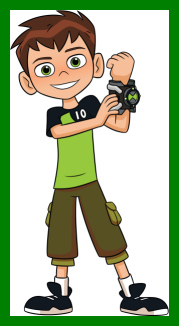
\includegraphics[width=14.69in]{Apresentação_files/figure-latex/unnamed-chunk-6-1}

\hypertarget{corte-de-bordas}{%
\section{Corte de bordas}\label{corte-de-bordas}}

\begin{Shaded}
\begin{Highlighting}[]
\FunctionTok{image\_trim}\NormalTok{(ben10, }\AttributeTok{fuzz=}\DecValTok{50}\NormalTok{)}
\end{Highlighting}
\end{Shaded}

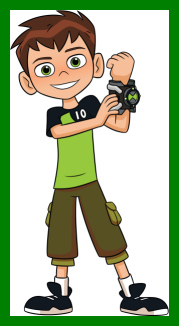
\includegraphics[width=2.21in]{Apresentação_files/figure-latex/unnamed-chunk-7-1}

\hypertarget{crop-images}{%
\section{Crop images}\label{crop-images}}

\begin{Shaded}
\begin{Highlighting}[]
\FunctionTok{image\_crop}\NormalTok{(ben10, }\StringTok{"150x130"}\NormalTok{)}
\end{Highlighting}
\end{Shaded}


\includegraphics[width=2.08in]{Apresentação_files/figure-latex/unnamed-chunk-8-1}

\hypertarget{rotauxe7uxe3o-e-espelhamento}{%
\section{Rotação e espelhamento}\label{rotauxe7uxe3o-e-espelhamento}}

\begin{Shaded}
\begin{Highlighting}[]
\FunctionTok{image\_rotate}\NormalTok{(ben10, }\DecValTok{45}\NormalTok{)}
\end{Highlighting}
\end{Shaded}


\includegraphics[width=4.6in]{Apresentação_files/figure-latex/unnamed-chunk-9-1}

\begin{Shaded}
\begin{Highlighting}[]
\FunctionTok{image\_flip}\NormalTok{(ben10)}
\end{Highlighting}
\end{Shaded}


\includegraphics[width=2.21in]{Apresentação_files/figure-latex/unnamed-chunk-10-1}

\begin{Shaded}
\begin{Highlighting}[]
\FunctionTok{image\_flop}\NormalTok{(ben10)}
\end{Highlighting}
\end{Shaded}


\includegraphics[width=2.21in]{Apresentação_files/figure-latex/unnamed-chunk-11-1}

\hypertarget{modulauxe7uxe3o-e-pintura}{%
\section{Modulação e pintura}\label{modulauxe7uxe3o-e-pintura}}

\begin{Shaded}
\begin{Highlighting}[]
\FunctionTok{image\_modulate}\NormalTok{(ben10, }\AttributeTok{brightness =} \DecValTok{100}\NormalTok{, }\AttributeTok{saturation =} \DecValTok{200}\NormalTok{, }\AttributeTok{hue =} \DecValTok{100}\NormalTok{)}
\end{Highlighting}
\end{Shaded}


\includegraphics[width=2.21in]{Apresentação_files/figure-latex/unnamed-chunk-12-1}

\begin{Shaded}
\begin{Highlighting}[]
\FunctionTok{image\_fill}\NormalTok{(ben10, }\StringTok{"blue"}\NormalTok{, }\AttributeTok{point =} \StringTok{"+50+200"}\NormalTok{, }\AttributeTok{fuzz =} \DecValTok{20}\NormalTok{)}
\end{Highlighting}
\end{Shaded}

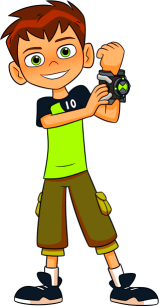
\includegraphics[width=2.21in]{Apresentação_files/figure-latex/unnamed-chunk-13-1}

\hypertarget{anotauxe7uxf5es-de-texto}{%
\section{Anotações de texto}\label{anotauxe7uxf5es-de-texto}}

\begin{Shaded}
\begin{Highlighting}[]
\FunctionTok{image\_annotate}\NormalTok{(ben10, }\AttributeTok{text =} \StringTok{"Ben 10"}\NormalTok{, }\AttributeTok{size =} \DecValTok{20}\NormalTok{,}
               \AttributeTok{degrees =} \SpecialCharTok{{-}}\DecValTok{10}\NormalTok{, }\AttributeTok{font =} \StringTok{"Georgia"}\NormalTok{,}
               \AttributeTok{color =} \StringTok{"green"}\NormalTok{,}
               \AttributeTok{location =} \StringTok{"+40+135"}\NormalTok{,}
               \AttributeTok{style =} \StringTok{"italic"}\NormalTok{, }
               \AttributeTok{boxcolor =} \StringTok{"lightblue"}\NormalTok{)}
\end{Highlighting}
\end{Shaded}

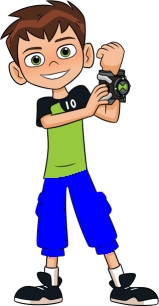
\includegraphics[width=2.21in]{Apresentação_files/figure-latex/unnamed-chunk-14-1}

\hypertarget{sobreposiuxe7uxe3o-de-imagens}{%
\section{Sobreposição de imagens}\label{sobreposiuxe7uxe3o-de-imagens}}

\begin{Shaded}
\begin{Highlighting}[]
\NormalTok{bigdata }\OtherTok{\textless{}{-}} \FunctionTok{image\_read}\NormalTok{(}\StringTok{"C:/Users/User/OneDrive {-} unb.br/Documentos/Manipulação de imagens/images/bigdata.jpg"}\NormalTok{)}
\NormalTok{rlogo }\OtherTok{\textless{}{-}} \FunctionTok{image\_read}\NormalTok{(}\StringTok{"C:/Users/User/OneDrive {-} unb.br/Documentos/Manipulação de imagens/images/Rlogo.jpg"}\NormalTok{)}
\NormalTok{sobre }\OtherTok{\textless{}{-}} \FunctionTok{c}\NormalTok{(bigdata,rlogo, ben10)}
\NormalTok{sobre }\OtherTok{\textless{}{-}} \FunctionTok{image\_scale}\NormalTok{(sobre, }\StringTok{"300x300"}\NormalTok{)}
\FunctionTok{image\_info}\NormalTok{(sobre)}
\end{Highlighting}
\end{Shaded}

\begin{verbatim}
##   format width height colorspace matte filesize density
## 1   JPEG   300    134       sRGB FALSE        0   72x72
## 2    PNG   300    228       sRGB  TRUE        0 118x118
## 3    PNG   156    300       sRGB  TRUE        0   28x28
\end{verbatim}

\begin{Shaded}
\begin{Highlighting}[]
\FunctionTok{image\_mosaic}\NormalTok{(sobre)}
\end{Highlighting}
\end{Shaded}

\includegraphics[width=4.17in]{Apresentação_files/figure-latex/unnamed-chunk-16-1}

\hypertarget{crie-uma-uxfanica-imagem-que-tenha-o-tamanho-da-primeira-imagem}{%
\subsection{Crie uma única imagem que tenha o tamanho da primeira
imagem}\label{crie-uma-uxfanica-imagem-que-tenha-o-tamanho-da-primeira-imagem}}

\begin{Shaded}
\begin{Highlighting}[]
\FunctionTok{image\_flatten}\NormalTok{(sobre)}
\end{Highlighting}
\end{Shaded}

\includegraphics[width=4.17in]{Apresentação_files/figure-latex/unnamed-chunk-17-1}
\#\# Adicionando imagens

\begin{Shaded}
\begin{Highlighting}[]
\FunctionTok{image\_flatten}\NormalTok{(sobre, }\StringTok{"add"}\NormalTok{)}
\end{Highlighting}
\end{Shaded}

\includegraphics[width=4.17in]{Apresentação_files/figure-latex/unnamed-chunk-18-1}
\#\# Modulate

\begin{Shaded}
\begin{Highlighting}[]
\FunctionTok{image\_flatten}\NormalTok{(sobre, }\StringTok{"modulate"}\NormalTok{)}
\end{Highlighting}
\end{Shaded}

\includegraphics[width=4.17in]{Apresentação_files/figure-latex/unnamed-chunk-19-1}
\#\# Minus

\begin{Shaded}
\begin{Highlighting}[]
\FunctionTok{image\_flatten}\NormalTok{(sobre, }\StringTok{"minus"}\NormalTok{)}
\end{Highlighting}
\end{Shaded}

\includegraphics[width=4.17in]{Apresentação_files/figure-latex/unnamed-chunk-20-1}
\#\# Colocando imagens uma ao lado de outra

\begin{Shaded}
\begin{Highlighting}[]
\FunctionTok{image\_append}\NormalTok{(}\FunctionTok{image\_scale}\NormalTok{(sobre, }\StringTok{"x200"}\NormalTok{))}
\end{Highlighting}
\end{Shaded}

\includegraphics[width=11.32in]{Apresentação_files/figure-latex/unnamed-chunk-21-1}
\# Empilhando

\begin{Shaded}
\begin{Highlighting}[]
\FunctionTok{image\_append}\NormalTok{(}\FunctionTok{image\_scale}\NormalTok{(sobre, }\StringTok{"100"}\NormalTok{), }\AttributeTok{stack =} \ConstantTok{TRUE}\NormalTok{) }
\end{Highlighting}
\end{Shaded}

\includegraphics[width=1.39in]{Apresentação_files/figure-latex/unnamed-chunk-22-1}
\# Combinar imagens em posições específicas

\begin{Shaded}
\begin{Highlighting}[]
\NormalTok{bigdataben10 }\OtherTok{\textless{}{-}} \FunctionTok{image\_scale}\NormalTok{(}\FunctionTok{image\_rotate}\NormalTok{(}\FunctionTok{image\_background}\NormalTok{(ben10, }\StringTok{"none"}\NormalTok{), }\DecValTok{400}\NormalTok{), }\StringTok{"x200"}\NormalTok{)}
\FunctionTok{image\_composite}\NormalTok{(}\FunctionTok{image\_scale}\NormalTok{(bigdata, }\StringTok{"x300"}\NormalTok{), bigdataben10, }\AttributeTok{offset =} \StringTok{"+200+50"}\NormalTok{)}
\end{Highlighting}
\end{Shaded}

\includegraphics[width=9.36in]{Apresentação_files/figure-latex/unnamed-chunk-23-1}

\hypertarget{alguns-efeitos}{%
\subsection{Alguns efeitos}\label{alguns-efeitos}}

\begin{Shaded}
\begin{Highlighting}[]
\FunctionTok{image\_oilpaint}\NormalTok{(ben10, }\AttributeTok{radius =} \DecValTok{1}\NormalTok{)}
\end{Highlighting}
\end{Shaded}

\includegraphics[width=2.21in]{Apresentação_files/figure-latex/unnamed-chunk-24-1}

\begin{Shaded}
\begin{Highlighting}[]
\FunctionTok{image\_implode}\NormalTok{(ben10, }\AttributeTok{factor =} \FloatTok{0.5}\NormalTok{)}
\end{Highlighting}
\end{Shaded}

\includegraphics[width=2.21in]{Apresentação_files/figure-latex/unnamed-chunk-25-1}

\begin{Shaded}
\begin{Highlighting}[]
\FunctionTok{image\_charcoal}\NormalTok{(ben10, }\AttributeTok{radius =} \DecValTok{1}\NormalTok{, }\AttributeTok{sigma =} \FloatTok{0.5}\NormalTok{)}
\end{Highlighting}
\end{Shaded}

\includegraphics[width=2.21in]{Apresentação_files/figure-latex/unnamed-chunk-26-1}

\begin{Shaded}
\begin{Highlighting}[]
\FunctionTok{image\_blur}\NormalTok{(ben10, }\AttributeTok{radius =} \DecValTok{1}\NormalTok{, }\AttributeTok{sigma =} \FloatTok{0.5}\NormalTok{)}
\end{Highlighting}
\end{Shaded}

\includegraphics[width=2.21in]{Apresentação_files/figure-latex/unnamed-chunk-27-1}

\begin{Shaded}
\begin{Highlighting}[]
\FunctionTok{image\_edge}\NormalTok{(ben10, }\AttributeTok{radius =} \DecValTok{1}\NormalTok{)}
\end{Highlighting}
\end{Shaded}

\includegraphics[width=2.21in]{Apresentação_files/figure-latex/unnamed-chunk-28-1}

\begin{Shaded}
\begin{Highlighting}[]
\FunctionTok{image\_negate}\NormalTok{(ben10)}
\end{Highlighting}
\end{Shaded}

\includegraphics[width=2.21in]{Apresentação_files/figure-latex/unnamed-chunk-29-1}

\begin{Shaded}
\begin{Highlighting}[]
\FunctionTok{image\_noise}\NormalTok{(ben10, }\AttributeTok{noisetype =} \StringTok{"uniform"}\NormalTok{)}
\end{Highlighting}
\end{Shaded}

\includegraphics[width=2.21in]{Apresentação_files/figure-latex/unnamed-chunk-30-1}

\begin{Shaded}
\begin{Highlighting}[]
\FunctionTok{image\_noise}\NormalTok{(ben10, }\AttributeTok{noisetype =} \StringTok{"Multiplicative Gaussian"}\NormalTok{)}
\end{Highlighting}
\end{Shaded}

\includegraphics[width=2.21in]{Apresentação_files/figure-latex/unnamed-chunk-31-1}

\hypertarget{criauxe7uxe3o-de-gifs}{%
\section{Criação de GIFs}\label{criauxe7uxe3o-de-gifs}}

\hypertarget{alguns-recursos-do-pacote-imager}{%
\section{Alguns recursos do pacote
imager}\label{alguns-recursos-do-pacote-imager}}

\hypertarget{lendo-uma-imagem}{%
\section{Lendo uma imagem}\label{lendo-uma-imagem}}

\begin{Shaded}
\begin{Highlighting}[]
\FunctionTok{library}\NormalTok{(}\StringTok{"imager"}\NormalTok{)}
\NormalTok{ocean }\OtherTok{\textless{}{-}} \FunctionTok{load.image}\NormalTok{(}\StringTok{"C:/Users/User/OneDrive {-} unb.br/Documentos/Manipulação de imagens/images/ocean.jpg"}\NormalTok{)}
\FunctionTok{plot}\NormalTok{(ocean)}
\end{Highlighting}
\end{Shaded}

\includegraphics{Apresentação_files/figure-latex/unnamed-chunk-32-1.pdf}

\hypertarget{quadtrees}{%
\section{Quadtrees}\label{quadtrees}}

\begin{Shaded}
\begin{Highlighting}[]
\FunctionTok{library}\NormalTok{(imager)}
\FunctionTok{library}\NormalTok{(purrr)}
\end{Highlighting}
\end{Shaded}

\begin{verbatim}
## 
## Attaching package: 'purrr'
\end{verbatim}

\begin{verbatim}
## The following object is masked from 'package:magrittr':
## 
##     set_names
\end{verbatim}

\begin{Shaded}
\begin{Highlighting}[]
\NormalTok{ocn }\OtherTok{\textless{}{-}} \FunctionTok{load.image}\NormalTok{(}\StringTok{"C:}\SpecialCharTok{\textbackslash{}\textbackslash{}}\StringTok{Users}\SpecialCharTok{\textbackslash{}\textbackslash{}}\StringTok{User}\SpecialCharTok{\textbackslash{}\textbackslash{}}\StringTok{OneDrive {-} unb.br}\SpecialCharTok{\textbackslash{}\textbackslash{}}\StringTok{Documentos}\SpecialCharTok{\textbackslash{}\textbackslash{}}\StringTok{Manipulação de imagens}\SpecialCharTok{\textbackslash{}\textbackslash{}}\StringTok{images}\SpecialCharTok{\textbackslash{}\textbackslash{}}\StringTok{ocean.jpg"}\NormalTok{) }\SpecialCharTok{\%\textgreater{}\%} \FunctionTok{imresize}\NormalTok{(.}\DecValTok{5}\NormalTok{)}

\CommentTok{\#Dividir ao longo de x, e depois y}
\NormalTok{qsplit }\OtherTok{\textless{}{-}} \ControlFlowTok{function}\NormalTok{(ocn)}
\NormalTok{\{}
    \FunctionTok{imsplit}\NormalTok{(ocn,}\StringTok{"x"}\NormalTok{,}\DecValTok{2}\NormalTok{) }\SpecialCharTok{\%\textgreater{}\%} \FunctionTok{map}\NormalTok{(}\SpecialCharTok{\textasciitilde{}} \FunctionTok{imsplit}\NormalTok{(.,}\StringTok{"y"}\NormalTok{,}\DecValTok{2}\NormalTok{)) }\SpecialCharTok{\%\textgreater{}\%}
\NormalTok{        flatten }
\NormalTok{\}}

\FunctionTok{qsplit}\NormalTok{(ocn) }\SpecialCharTok{\%\textgreater{}\%}\NormalTok{ as.imlist }\SpecialCharTok{\%\textgreater{}\%}\NormalTok{ plot}
\end{Highlighting}
\end{Shaded}

\includegraphics{Apresentação_files/figure-latex/unnamed-chunk-33-1.pdf}

A operação inversa usa ``imappend'':

\begin{Shaded}
\begin{Highlighting}[]
\NormalTok{qunsplit }\OtherTok{\textless{}{-}} \ControlFlowTok{function}\NormalTok{(l)}
\NormalTok{\{}
    \FunctionTok{list}\NormalTok{(l[}\DecValTok{1}\SpecialCharTok{:}\DecValTok{2}\NormalTok{],l[}\DecValTok{3}\SpecialCharTok{:}\DecValTok{4}\NormalTok{]) }\SpecialCharTok{\%\textgreater{}\%} \FunctionTok{map}\NormalTok{(}\SpecialCharTok{\textasciitilde{}} \FunctionTok{imappend}\NormalTok{(.,}\StringTok{"y"}\NormalTok{)) }\SpecialCharTok{\%\textgreater{}\%} \FunctionTok{imappend}\NormalTok{(}\StringTok{"x"}\NormalTok{)}
\NormalTok{\}}

\FunctionTok{qsplit}\NormalTok{(ocn) }\SpecialCharTok{\%\textgreater{}\%}\NormalTok{ qunsplit }\SpecialCharTok{\%\textgreater{}\%}\NormalTok{ plot}
\end{Highlighting}
\end{Shaded}

\includegraphics{Apresentação_files/figure-latex/unnamed-chunk-34-1.pdf}

\begin{Shaded}
\begin{Highlighting}[]
\CommentTok{\#Max std. dev imoss channels}
\NormalTok{imsd }\OtherTok{\textless{}{-}} \ControlFlowTok{function}\NormalTok{(ocn)}
\NormalTok{\{}
    \FunctionTok{imsplit}\NormalTok{(ocn,}\StringTok{"c"}\NormalTok{) }\SpecialCharTok{\%\textgreater{}\%} \FunctionTok{map\_dbl}\NormalTok{(sd) }\SpecialCharTok{\%\textgreater{}\%}\NormalTok{ max}
\NormalTok{\}}
\end{Highlighting}
\end{Shaded}

\begin{Shaded}
\begin{Highlighting}[]
\NormalTok{refine }\OtherTok{\textless{}{-}} \ControlFlowTok{function}\NormalTok{(l)}
\NormalTok{\{}
    \ControlFlowTok{if}\NormalTok{ (}\FunctionTok{is.cimg}\NormalTok{(l)) }\CommentTok{\#We have a leaf}
\NormalTok{    \{}
\NormalTok{        qs }\OtherTok{\textless{}{-}} \FunctionTok{qsplit}\NormalTok{(l) }\CommentTok{\#Split}
        \ControlFlowTok{if}\NormalTok{ (}\FunctionTok{any}\NormalTok{(}\FunctionTok{dim}\NormalTok{(l)[}\DecValTok{1}\SpecialCharTok{:}\DecValTok{2}\NormalTok{] }\SpecialCharTok{\textless{}=} \DecValTok{4}\NormalTok{)) }\CommentTok{\#Quadrants are very small}
\NormalTok{        \{}
\NormalTok{            qs}\SpecialCharTok{$}\NormalTok{sds }\OtherTok{\textless{}{-}} \FunctionTok{rep}\NormalTok{(}\DecValTok{0}\NormalTok{,}\DecValTok{4}\NormalTok{) }\CommentTok{\#Prevent further refinement}
\NormalTok{        \}}
        \ControlFlowTok{else}
\NormalTok{        \{}
\NormalTok{            qs}\SpecialCharTok{$}\NormalTok{sds }\OtherTok{\textless{}{-}} \FunctionTok{map\_dbl}\NormalTok{(qs,imsd) }\CommentTok{\#Store std.dev of children}
\NormalTok{        \}}
\NormalTok{        qs}
\NormalTok{    \}}
    \ControlFlowTok{else} \CommentTok{\#Not a leaf, explore further}
\NormalTok{    \{}
\NormalTok{        indm }\OtherTok{\textless{}{-}} \FunctionTok{which.max}\NormalTok{(l}\SpecialCharTok{$}\NormalTok{sds) }\CommentTok{\#Find child with max. std. dev}
\NormalTok{        l[[indm]] }\OtherTok{\textless{}{-}} \FunctionTok{refine}\NormalTok{(l[[indm]]) }\CommentTok{\#Refine}
\NormalTok{        l}\SpecialCharTok{$}\NormalTok{sds[indm] }\OtherTok{\textless{}{-}} \FunctionTok{max}\NormalTok{(l[[indm]]}\SpecialCharTok{$}\NormalTok{sds) }\CommentTok{\#Update std. dev}
\NormalTok{        l}
\NormalTok{    \}}
\NormalTok{\}}
\end{Highlighting}
\end{Shaded}

\begin{Shaded}
\begin{Highlighting}[]
\NormalTok{rebuild }\OtherTok{\textless{}{-}} \ControlFlowTok{function}\NormalTok{(l,}\AttributeTok{borders=}\ConstantTok{FALSE}\NormalTok{)}
\NormalTok{\{}
    \FunctionTok{map}\NormalTok{(l[}\SpecialCharTok{{-}}\DecValTok{5}\NormalTok{],}\SpecialCharTok{\textasciitilde{}} \ControlFlowTok{if}\NormalTok{ (}\FunctionTok{is.cimg}\NormalTok{(.)) }\FunctionTok{meanim}\NormalTok{(.,}\AttributeTok{borders=}\NormalTok{borders) }\ControlFlowTok{else} \FunctionTok{rebuild}\NormalTok{(.,}\AttributeTok{borders=}\NormalTok{borders)) }\SpecialCharTok{\%\textgreater{}\%}\NormalTok{ qunsplit}
\NormalTok{\}}

\CommentTok{\#Produce an image that\textquotesingle{}s just the average of image im}
\CommentTok{\#Optionally, add borders}
\NormalTok{meanim }\OtherTok{\textless{}{-}} \ControlFlowTok{function}\NormalTok{(ocn,}\AttributeTok{borders=}\ConstantTok{FALSE}\NormalTok{)}
\NormalTok{\{}
\NormalTok{    ocn }\OtherTok{\textless{}{-}} \FunctionTok{imsplit}\NormalTok{(ocn,}\StringTok{"c"}\NormalTok{) }\SpecialCharTok{\%\textgreater{}\%} \FunctionTok{map}\NormalTok{(}\SpecialCharTok{\textasciitilde{}} \DecValTok{0}\SpecialCharTok{*}\NormalTok{. }\SpecialCharTok{+} \FunctionTok{mean}\NormalTok{(.)) }\SpecialCharTok{\%\textgreater{}\%} \FunctionTok{imappend}\NormalTok{(}\StringTok{"c"}\NormalTok{)}
    \ControlFlowTok{if}\NormalTok{ (borders)}
\NormalTok{    \{}
\NormalTok{        ocn[}\FunctionTok{px.borders}\NormalTok{(ocn)] }\OtherTok{\textless{}{-}} \DecValTok{0}
\NormalTok{    \}}
\NormalTok{    ocn}
\NormalTok{\}}
\end{Highlighting}
\end{Shaded}

\begin{Shaded}
\begin{Highlighting}[]
\NormalTok{iter.refine }\OtherTok{\textless{}{-}} \ControlFlowTok{function}\NormalTok{(ocn,nIter)}
\NormalTok{\{}
    \ControlFlowTok{for}\NormalTok{ (i }\ControlFlowTok{in} \FunctionTok{seq\_len}\NormalTok{(nIter)) \{ ocn }\OtherTok{\textless{}{-}} \FunctionTok{refine}\NormalTok{(ocn) \};}
\NormalTok{    ocn}
\NormalTok{\}}

\CommentTok{\#The first four iterations of the process}
\FunctionTok{map\_il}\NormalTok{(}\DecValTok{1}\SpecialCharTok{:}\DecValTok{4}\NormalTok{,}\SpecialCharTok{\textasciitilde{}} \FunctionTok{iter.refine}\NormalTok{(ocn,.) }\SpecialCharTok{\%\textgreater{}\%}\NormalTok{ rebuild) }\SpecialCharTok{\%\textgreater{}\%}\NormalTok{ plot}
\end{Highlighting}
\end{Shaded}

\includegraphics{Apresentação_files/figure-latex/unnamed-chunk-38-1.pdf}

\begin{Shaded}
\begin{Highlighting}[]
\FunctionTok{iter.refine}\NormalTok{(ocn,}\DecValTok{1000}\NormalTok{) }\SpecialCharTok{\%\textgreater{}\%} \FunctionTok{rebuild}\NormalTok{(}\AttributeTok{borders=}\NormalTok{T) }\SpecialCharTok{\%\textgreater{}\%}\NormalTok{ plot}
\end{Highlighting}
\end{Shaded}

\includegraphics{Apresentação_files/figure-latex/unnamed-chunk-39-1.pdf}

\hypertarget{embaralhar-colunas-de-uma-imagem-e-colocuxe1-la-de-volta}{%
\section{Embaralhar colunas de uma imagem, e colocá-la de
volta}\label{embaralhar-colunas-de-uma-imagem-e-colocuxe1-la-de-volta}}

\begin{Shaded}
\begin{Highlighting}[]
\FunctionTok{library}\NormalTok{(imager)}
\FunctionTok{library}\NormalTok{(purrr)}
\FunctionTok{set.seed}\NormalTok{(}\DecValTok{2}\NormalTok{)}

\NormalTok{im }\OtherTok{\textless{}{-}} \FunctionTok{load.image}\NormalTok{(}\StringTok{"C:}\SpecialCharTok{\textbackslash{}\textbackslash{}}\StringTok{Users}\SpecialCharTok{\textbackslash{}\textbackslash{}}\StringTok{User}\SpecialCharTok{\textbackslash{}\textbackslash{}}\StringTok{OneDrive {-} unb.br}\SpecialCharTok{\textbackslash{}\textbackslash{}}\StringTok{Documentos}\SpecialCharTok{\textbackslash{}\textbackslash{}}\StringTok{Manipulação de imagens}\SpecialCharTok{\textbackslash{}\textbackslash{}}\StringTok{images}\SpecialCharTok{\textbackslash{}\textbackslash{}}\StringTok{acropolis.jpg"}\NormalTok{)}

\DocumentationTok{\#\#reorder the columns of an image}
\NormalTok{scramble }\OtherTok{\textless{}{-}} \ControlFlowTok{function}\NormalTok{(im)}
\NormalTok{\{}
    \FunctionTok{imsplit}\NormalTok{(im,}\StringTok{"x"}\NormalTok{) }\SpecialCharTok{\%\textgreater{}\%}\NormalTok{ \{ .[}\FunctionTok{sample}\NormalTok{(}\FunctionTok{length}\NormalTok{(.))] \} }\SpecialCharTok{\%\textgreater{}\%} \FunctionTok{imappend}\NormalTok{(}\StringTok{"x"}\NormalTok{) }
\NormalTok{\}}
\FunctionTok{scramble}\NormalTok{(im) }\SpecialCharTok{\%\textgreater{}\%}\NormalTok{ plot}
\end{Highlighting}
\end{Shaded}

\includegraphics{Apresentação_files/figure-latex/unnamed-chunk-40-1.pdf}

\begin{Shaded}
\begin{Highlighting}[]
\FunctionTok{imlist}\NormalTok{(im,}\FunctionTok{scramble}\NormalTok{(im)) }\SpecialCharTok{\%\textgreater{}\%} \FunctionTok{plot}\NormalTok{(}\AttributeTok{layout=}\StringTok{"row"}\NormalTok{)}
\end{Highlighting}
\end{Shaded}

\includegraphics{Apresentação_files/figure-latex/unnamed-chunk-41-1.pdf}

\begin{Shaded}
\begin{Highlighting}[]
\FunctionTok{library}\NormalTok{(seriation)}

\NormalTok{unscramble }\OtherTok{\textless{}{-}} \ControlFlowTok{function}\NormalTok{(im.s,}\AttributeTok{method=}\StringTok{"TSP"}\NormalTok{,...)}
\NormalTok{\{}
\NormalTok{    cols }\OtherTok{\textless{}{-}} \FunctionTok{imsplit}\NormalTok{(im.s,}\StringTok{"x"}\NormalTok{)}
    \CommentTok{\#Compute a distance matrix (using L1 {-} Manhattan {-} distance)}
    \CommentTok{\#Each entry D\_ij compares column i to column j  }
\NormalTok{    D }\OtherTok{\textless{}{-}} \FunctionTok{map}\NormalTok{(cols,as.vector) }\SpecialCharTok{\%\textgreater{}\%} \FunctionTok{do.call}\NormalTok{(rbind,.) }\SpecialCharTok{\%\textgreater{}\%} \FunctionTok{dist}\NormalTok{(}\AttributeTok{method=}\StringTok{"manhattan"}\NormalTok{)}
\NormalTok{    out }\OtherTok{\textless{}{-}} \FunctionTok{seriate}\NormalTok{(D,}\AttributeTok{method=}\NormalTok{method,...)}
\NormalTok{    cols[}\FunctionTok{get\_order}\NormalTok{(out)] }\SpecialCharTok{\%\textgreater{}\%} \FunctionTok{imappend}\NormalTok{(}\StringTok{"x"}\NormalTok{) }
\NormalTok{\}}

\FunctionTok{scramble}\NormalTok{(im) }\SpecialCharTok{\%\textgreater{}\%}\NormalTok{ unscramble }\SpecialCharTok{\%\textgreater{}\%} \FunctionTok{plot}\NormalTok{(}\AttributeTok{main=}\StringTok{"Unscrambled image"}\NormalTok{)}
\end{Highlighting}
\end{Shaded}

\includegraphics{Apresentação_files/figure-latex/unnamed-chunk-42-1.pdf}

\begin{Shaded}
\begin{Highlighting}[]
\NormalTok{scramble }\OtherTok{\textless{}{-}} \ControlFlowTok{function}\NormalTok{(im,}\AttributeTok{axis=}\StringTok{"x"}\NormalTok{)}
\NormalTok{\{}
    \FunctionTok{imsplit}\NormalTok{(im,axis) }\SpecialCharTok{\%\textgreater{}\%}\NormalTok{ \{ .[}\FunctionTok{sample}\NormalTok{(}\FunctionTok{length}\NormalTok{(.))] \} }\SpecialCharTok{\%\textgreater{}\%} \FunctionTok{imappend}\NormalTok{(axis) }
\NormalTok{\}}


\NormalTok{unscramble }\OtherTok{\textless{}{-}} \ControlFlowTok{function}\NormalTok{(im,}\AttributeTok{axis=}\StringTok{"x"}\NormalTok{,}\AttributeTok{method=}\StringTok{"TSP"}\NormalTok{,...)}
\NormalTok{\{}
\NormalTok{    cols }\OtherTok{\textless{}{-}} \FunctionTok{imsplit}\NormalTok{(im,axis)}
    \CommentTok{\#Compute a distance matrix (using L1 {-} Manhattan {-} distance)}
    \CommentTok{\#Each entry D\_ij compares column i to column j  }
\NormalTok{    D }\OtherTok{\textless{}{-}} \FunctionTok{map}\NormalTok{(cols,as.vector) }\SpecialCharTok{\%\textgreater{}\%} \FunctionTok{do.call}\NormalTok{(rbind,.) }\SpecialCharTok{\%\textgreater{}\%} \FunctionTok{dist}\NormalTok{(}\AttributeTok{method=}\StringTok{"manhattan"}\NormalTok{)}
\NormalTok{    out }\OtherTok{\textless{}{-}} \FunctionTok{seriate}\NormalTok{(D,}\AttributeTok{method=}\NormalTok{method,...)}
\NormalTok{    cols[}\FunctionTok{get\_order}\NormalTok{(out)] }\SpecialCharTok{\%\textgreater{}\%} \FunctionTok{imappend}\NormalTok{(axis) }
\NormalTok{\}}

\NormalTok{im }\OtherTok{\textless{}{-}} \FunctionTok{scramble}\NormalTok{(im,}\StringTok{"x"}\NormalTok{) }\SpecialCharTok{\%\textgreater{}\%} \FunctionTok{scramble}\NormalTok{(}\StringTok{"y"}\NormalTok{)}

\CommentTok{\#The double scramble produces an unrecognisable mess}
\FunctionTok{plot}\NormalTok{(im)}
\end{Highlighting}
\end{Shaded}

\includegraphics{Apresentação_files/figure-latex/unnamed-chunk-43-1.pdf}

\begin{Shaded}
\begin{Highlighting}[]
\FunctionTok{unscramble}\NormalTok{(im,}\StringTok{"y"}\NormalTok{) }\SpecialCharTok{\%\textgreater{}\%} \FunctionTok{unscramble}\NormalTok{(}\StringTok{"x"}\NormalTok{) }\SpecialCharTok{\%\textgreater{}\%}\NormalTok{ plot}
\end{Highlighting}
\end{Shaded}

\includegraphics{Apresentação_files/figure-latex/unnamed-chunk-44-1.pdf}

\hypertarget{referencias-bibliogruxe1ficas}{%
\subsection{Referencias
bibliográficas}\label{referencias-bibliogruxe1ficas}}

\end{document}
